\section{Mitosis-Stream}\label{chap:mitosis-stream}
Mitosis-Stream is enhancing the Mitosis-Core with video streaming functionality. While Mitosis-Core is responsible for setting up an overlay network, the Mitosis-Stream module is responsible to construct a \glsfirst{dag} of video streaming connections. The \gls{dag} is created on top of the existing overlay mesh network.

\begin{figure}
\centering
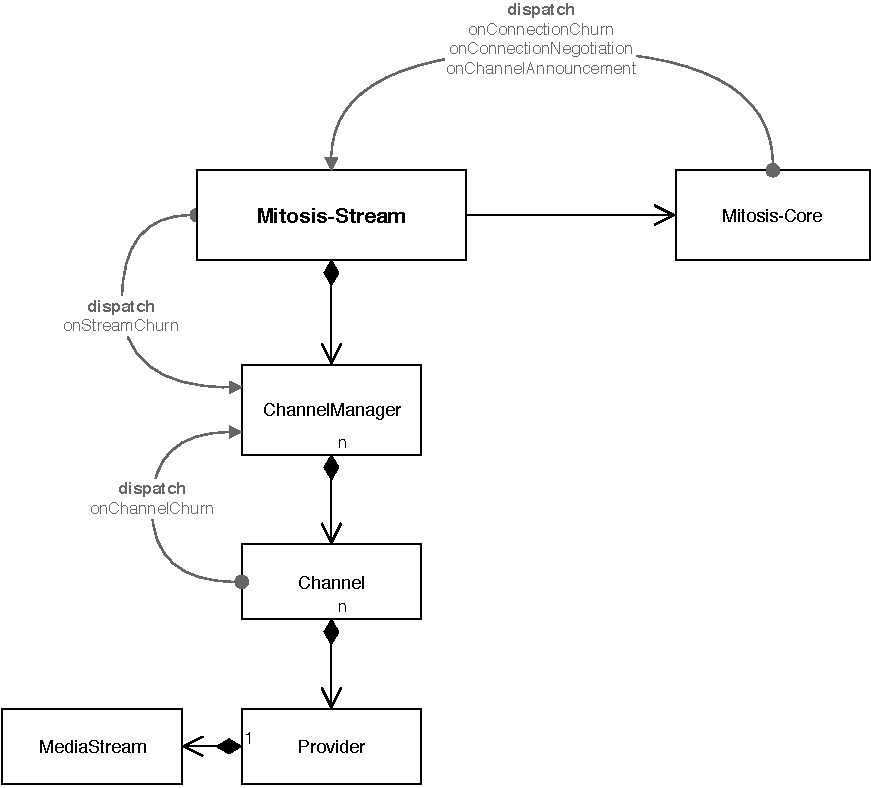
\includegraphics[width=0.75\textwidth]{graphics/implementation/mitosis-architecture-mitosis-stream.pdf}
\caption{Mitosis-Stream}
\label{fig:mit-stream}
\end{figure}

As presented in \vref{fig:mit-stream}, Mitosis-Stream brings its own components and interacts with Mitosis-Core via the given interface. 

\subsection{ChannelManager}
The \lstinline|ChannelManger| is the owner of all available \lstinline|Channels|. Through the ChannelManager new channels can be added.
There are three scenarios where a new channel is added.
\begin{enumerate}
    \itembf{User starts stream} The ChannelManager provides a method \lstinline|setLocalStream| and accepts a \lstinline|MediaStream| as argument. When the method is called the ChannelManager creates a new \lstinline|Channel| and adds the peer as a \lstinline|Provider|.
    \itembf{Stream-Connection is opened} When a new stream connection is opened the ChannelManager creates a new channel and adds the stream connection initiator as provider.
    \itembf{ChannelAnnouncement} On receipt of a \channelAnnouncement, a new channel is added with the peer who is announcing the channel as provider. If the channel has already been created the announcing peer is added as provider.
\end{enumerate}

\subsection{Channel and Provider}
A channel is the representation of a video broadcast circulating in the network. As the channel can be received by multiple peers, each peer providing a channel is represented as a provider. A provider is active when the peer has an open WebRTCStream connection and actively receives a \lstinline|MediaStream|. Each provider has a maximum of allowed WebRTCStream connections. The maximum is represented as capacity. For example, when a peer can open two additional WebRTCStream connections, it has a capacity of $\ 2 $.

\subsection{Push and Pull}
\vref{sec:design-stream-construction} described the two phases that create the streaming graph. The ChannelManager implements the push phase either if the user started a local channel or if an unsolicited stream connection was opened. The ChannelManager looks at neighbours with available stream capacity and filters out those who already provide the channel in question.
The second phase is implemented through the channel announcements. If a peer with inbound capacity is informed of a neighbour with outbound capacity, it actively sends a connection negotiation \lstinline|request| with the id of the channel it wants to acquire.
